\chapter{Preliminares}

En esta sección se presenta el marco teórico de este trabajo, dando un panorama
general de cada una de las disciplinas abordadas e introduciendo los conceptos
básicos y fundamentales para entender el proyecto. Se comienza con la definición
de la taxonomía del campo de estudio, luego \todo{describir las siguientes
secciones}

\section{Taxonomía del Campo de Estudio}

\begin{figure}
   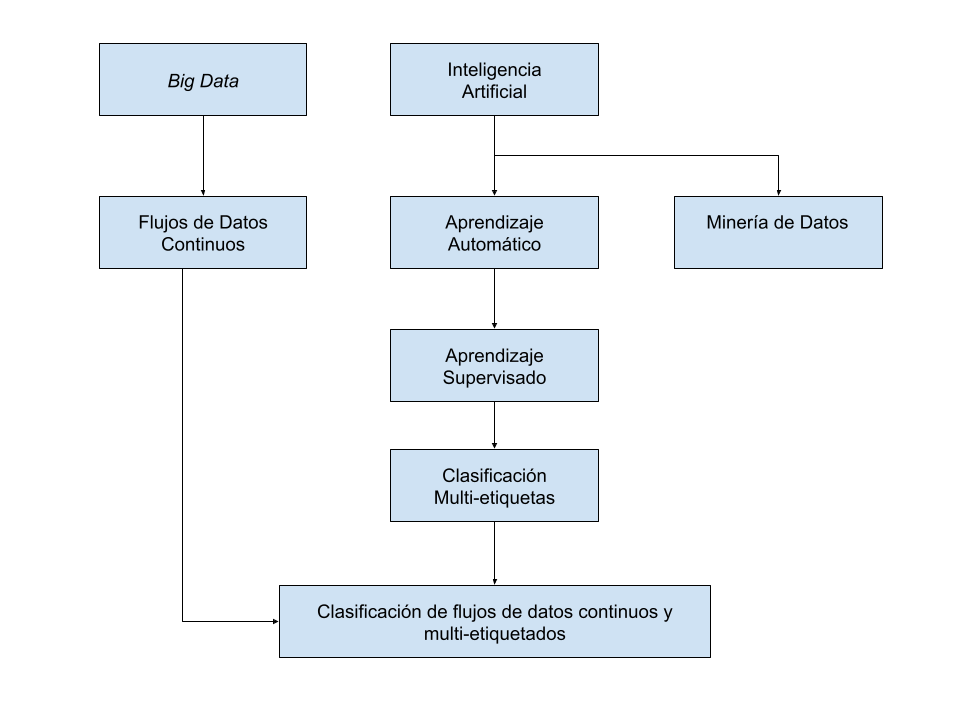
\includegraphics[width=.9\linewidth]{figures/study_field_taxonomy_v2.png}
   \centering
   \caption{Taxonomía del campo de estudio.}
   \label{fig:campo_estudio}
\end{figure}

En pocas palabras, el presente trabajo de investigación se enmarca en las áreas
de \textit{big data} y minería de datos, con aplicación en escenarios de
\textit{streaming} o flujos continuos de datos y abordando clasificaciones
multi-etiquetas. También se aprovechan técnicas del área de procesamiento de
lenguaje natural para tratar corpus de texto libre y extraer \textit{features} o
características representativas de los datos.

La figura \ref{fig:campo_estudio} es un esquema que ilustra la taxonomía del
campo de estudio y la interrelación entre las áreas de investigación
involucradas.

\section{Aprendizaje Automático}

El aprendizaje automático, también conocido por su término en ingles
“\textit{Machine Learning}”, se enmarca dentro del área de la \acrfull{ia} y
estudia cómo las computadoras pueden “aprender” o mejorar su rendimiento
meramente a partir de datos y sin la intervención de un ser humano.  La idea
detrás de esta disciplina es lograr reconocer patrones subyacentes en los datos
y tomar decisiones en base a estos. Por ejemplo, un problema de aprendizaje
automático es el de reconocer dígitos escritos a mano a partir de un conjunto de
ejemplos (ver figura \ref{fig:reconocimiento_digitos}).  Aquí se tienen un
conjunto de imágenes, cada una representando un dígito del 0 al 9, y el objetivo
es construir un modelo que sea capaz de detectar de qué dígito se trata. Otro
ejemplo es el de hallar documentos de texto que son relevantes a una consulta
del usuario. En este caso el modelo recibe un conjunto acotado de términos, los
cuales describen una necesidad de información del usuario, y el modelo debe ser
capaz de retornar los documentos que satisfacen la consulta.  

Estos problemas se suelen categorizar en aprendizaje supervisado o no
supervisado, de acuerdo a si se conoce o no de antemano el concepto o etiqueta
que define a los datos. Se desarrollará más sobre este punto en las próximas
secciones. De entre los problemas de aprendizaje supervisado se destaca aquí el
de clasificación, el cual será descrito a continuación.

\begin{figure}
   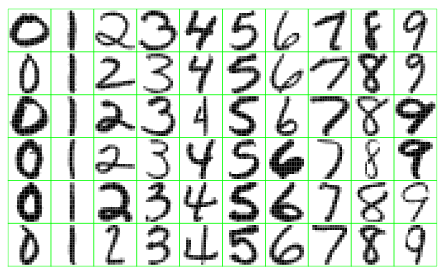
\includegraphics[width=0.66\linewidth]{figures/digits_recognition_v2.png}
   \centering
   \caption{Dígitos escritos a mano. Fuente: \citetitle{hastie_elements_2009}
   (\citeyear{hastie_elements_2009}).}
   \label{fig:reconocimiento_digitos}
\end{figure}

\section{Clasificación}

La clasificación es una tarea de minería de datos muy popular que consiste en
hallar modelos que describen la o las clases intrínsecas de los datos. La clase
corresponde a un concepto que representa al dato y es una etiqueta categórica,
es decir, un valor discreto de entre un conjunto de valores previamente
conocidos. Estos modelos, también llamados clasificadores, son capaces de
predecir la clase a la que corresponden datos previamente desconocidos. Por
ejemplo, se puede construir un modelo de clasificación para categorizar nuevos
correos electrónicos  de acuerdo a si se trata de correo basura (también
conocido como "\textit{spam}") o no. Dicho análisis puede ayudar a obtener un
mayor entendimiento de los datos a alto nivel. Las tareas de clasificación han
sido aplicadas en áreas tales como las de aprendizaje automático, reconocimiento
de patrones o estadística. En un principio, buena parte de los algoritmos se
ejecutaban en memoria, con la limitación de espacio de almacenamiento que eso
conlleva. Investigaciones más recientes han desarrollado técnicas para escalar
los algoritmos de tal manera que puedan manejar datos de mayor tamaño, alojados
en memoria, en disco o procesados bajo demanda. Las aplicaciones para este tipo
de tareas son numerosas y entre ellas se encuentran las de detectar fraudes o
realizar diagnósticos médicos, entre otras.

La clasificación de datos consta de dos etapas, una de aprendizaje y otra de
clasificación o predicción. Durante la tarea de aprendizaje se construye el
modelo de clasificación  el cual describe un determinado número de clases o
conceptos. También se conoce esta etapa como la de entrenamiento ya que se
selecciona un subconjunto de los datos, llamado conjunto de entrenamiento, que
consta de instancias o tuplas seleccionadas aleatoriamente y con una o más
etiquetas asociadas. Formalmente, el problema de clasificación puede ser
formulado de la siguiente manera. Se recibe un conjunto etiquetado de
instancias, tupas o ejemplos de la forma $( X, y )$ donde cada tupla es un
vector $X=(x_{1},x_{2},...,x_{n})$, siendo cada valor una característica
distintiva, atributo o feature de la instancia. El vector $y$ por su parte toma
un valor de entre $n$ clases diferentes.

Este tipo de tareas se engloban dentro del campo de aprendizaje supervisado ya
que para cada instancia la etiqueta es conocida de antemano, y es aprovechada
para guiar o, siguiendo la metáfora, “supervisar” el aprendizaje del
clasificador. Esta es la diferencia principal contra algoritmos de aprendizaje
no supervisado, en los cuales la etiqueta no es conocida y se deben aplicar
técnicas para salvar esta restricción.

La primera etapa de una clasificación puede ser vista también como el
aprendizaje de una función $y=f(X)$ que pueda predecir la clase $y$ para una
tupla $X$. Por ejemplo, $X$ podría ser un mensaje de correo y la etiqueta $y$ la
decisión de si se trata de un correo basura o no. Desde esta perspectiva
queremos aprender una función que sea capaz de distinguir las clases
subyacentes.  Usualmente, esta asociación es llevada a cabo por algoritmos de
aprendizaje, los cuales internamente usan funciones matemáticas o reglas de
decisión. Algunos ejemplos de este tipo de algoritmos son los árboles de
decisión, \textit{naive} bayes, perceptrón, entre otros.

En la segunda etapa el modelo es usado para clasificar. En primer lugar, se
calcula una métrica de evaluación, tal como la exactitud o \textit{accuracy}.
Durante la etapa de entrenamiento esta estimación puede ser imprecisa, tomando
un valor que tiende a ser “optimista” o que da un valor de exactitud mayor al
rendimiento real. Esto sucede porque el clasificador puede llegar a incorporar
anomalías particulares en el conjunto de datos de entrenamiento. Este fenómeno
es llamado sobreajuste u “\textit{overfit}” y una técnica para reducirlo es
separar de entre los datos un subconjunto de prueba o de \textit{testing} que no
se usa durante el entrenamiento y a partir del cual se realizan predicciones y
se calculan las métricas de evaluación. En este contexto, la tarea de evaluación
es fundamental ya que es la vía a partir de la cual se determina qué algoritmos
o técnicas son más apropiados que otros para un problema en particular. Además
provee la información necesaria para corregir o ajustar los parámetros de los
algoritmos y así obtener modelos más robustos.

En definitiva, ambos pasos se aplican consecutivamente con el objetivo de lograr
hallar un modelo capaz de predecir etiquetas en instancias nuevas y
desconocidas.

Retomando la primera etapa de la clasificación, se describen a continuación
algunos algoritmos para generar modelos y que son particularmente relevantes
para este trabajo de investigación.

\subsection{\textit{Naive} Bayes}

\textit{Naive} Bayes es un modelo de clasificación computacionalmente simple
pero cuyo rendimiento es competitivo contra otros modelos más complejos. Se dice
que es un clasificador estadístico ya que se basa en el teorema de Bayes. La
idea es computar una probabilidad para cada una de las clases, basada en los
atributos de la instancia y seleccionar aquella de mayor probabilidad. El
término “\textit{naive}” es el inglés para el término “\textit{ingenuo}” y nace
de la presunción que hace el algoritmo de que los atributos son independientes
entre sí, o condicionalmente independientes. Esta presunción raramente se cumple
en los escenarios donde se aplica pero contribuye a su simplicidad computacional
y a su velocidad durante el entrenamiento.

El teorema de Bayes se define formalmente de la siguiente manera:

\begin{equation}
   P(H \mid X) = \frac{P(X \mid H) P(H)}{P(X)}
\end{equation}

En esta ecuación, el vector $X$ es una tupla definida tal como en la sección
anterior y en términos bayesianos representa la “evidencia”. $P(X)$, por lo
tanto, es la probabilidad de que la tupla contenga los atributos que posee. Por
su parte, $H$ es la hipótesis de que la tupla pertenece a una determinada clase
y $P(H)$ su probabilidad. Esta es conocida como probabilidad “a priori”. De la
misma manera, $P(H|X)$ es la probabilidad de que la hipótesis $H$ sea cierta
bajo la evidencia $X$. A esta se la llama probabilidad “a posteriori” con $H$
condicionada por $X$ y es el valor que se quiere determinar en una tarea de
clasificación.  Finalmente, $P(X|H)$ indica la probabilidad de que la tupla tenga
unos atributos determinados dado que se satisface la hipótesis.

Por su parte, la fórmula de \textit{Naive} Bayes es similar:

\begin{equation}
   P(C_{i} \mid X) = P(X \mid C_{i}) P(C_{i})
\end{equation}

Aquí el término $P(X)$ es descartado ya que se asume constante para todas las
clases. La hipótesis $H$ es representada como $C_{i}$ que es un valor de la
tupla $C=(C_{1},C_{2},...,C_{m})$, donde $m$ es el número de clases. La
presunción “ingenua” es aplicada para el cálculo del término $P(X \mid C_{i})$
gracias a lo cual se puede definir de la siguiente manera:

\begin{equation} 
   P(X \mid C_{i}) = \prod\limits_{k=1}^n{P(x_{k} \mid C_{i})} =
   P(x_{1} \mid C_{i}) \times 
   P(x_{2} \mid C_{i}) \times ... \times 
   P(x_{n} \mid C_{i})   
\end{equation}

Finalmente, el modelo seleccionará la clase que maximice el valor de
probabilidad.  

Como se ha dicho anteriormente, la simplicidad, velocidad computacional y su
competitividad en métricas de exactitud hacen de \textit{Naive} Bayes un
algoritmo destacado en el campo de aprendizaje automático
\cite{wickramasinghe_naive_2020} y ha sido aplicado para problemas diversos,
tales como el de hallar errores en programas de computación
\cite{arar_feature_2017}, predecir enfermedades del corazón
\cite{dulhare_prediction_2018} o detectar ataques en una red de computadoras
\cite{kalutarage_detecting_2015}.


\subsection{Árboles de Decisión}

Los árboles de decisión son un modelo de clasificación que se destaca por ser de
fácil interpretación e intuitivo para el ser humano. De hecho, se puede generar
una representación gráfica del árbol generado para asistir a la comprensión del
del modelo y de cómo se comporta durante una predicción. En cuanto a su
estructura, un árbol de decisión contiene nodos, cada uno representando un
atributo de la colección. Estos nodos se conectan con otros nodos a partir de
enlaces o “ramas” que representan un valor o un rango de valores de ese
atributo. Los nodos de menor jerarquía son llamados “hojas” y contienen la clase
de la predicción, y el nodo de mayor jerarquía es llamado “raíz”. Al momento de
predecir una instancia nueva, la clasificación se realiza de la siguiente
manera:  se toma la instancia nueva, la cual no tiene una etiqueta asociada, y
los valores de sus atributos son comparados contra los del árbol, luego se traza
un camino desde el nodo raíz hasta la hoja que contiene una clase y dicha clase
es la predicción resultante. 

Los árboles de decisión se generan a partir de un algoritmo de inducción.
Existen varios de estos algoritmos pero todos son variantes que han sido
diseñadas bajo un misma principio: construir  el árbol de una manera
“voraz”\footnote{Se le llama voraz o \textit{greedy} a un algoritmo que busca
   hallar la opción óptima en cada paso y, de esta manera, alcanzar la solución
   general óptima para resolver un problema.  Esto lo diferencia de algoritmos
   como los de \textit{backtracking}, los cuales exploran distintas
posibilidades y pueden volver al inicio en búsqueda de una mejor solución},
comenzando desde el nodo raíz (conocido como enfoque \textit{top-down}) y
eligiendo en cada paso el atributo más informativo o que maximice alguna medida
de ganancia de información. 

Algunos de estos algoritmos son:

\begin{description} 

   \item[\acrshort{id3}] Son las siglas de \textit{\acrlong{id3}} y fue
      desarrollado en 1986 por Ross Quinlan. Consiste en crear un árbol de
      múltiples vías, buscando para cada nodo el atributo categórico que lance
      la mayor ganancia de información para las clases categóricas. Los árboles
      crecen en un tamaño máximo y luego se realiza el paso de poda para mejorar
      el poder de generalización del modelo sobre datos desconocidos.

   \item[C4.5] Es la evolución del algoritmo \acrshort{id3}. La principal mejora
      con respecto a su predecesor es que elimina la restricción de que los
      atributos deban ser categóricos. Esto lo consigue particionando el valor
      continuo en rangos o en un conjunto de intervalos discretos. C4.5
      convierte el árbol entrenado en conjuntos de reglas de decisión. 

   \item[\acrshort{cart}] Son las siglas de \acrlong{cart} y es un algoritmo muy
      similar al C4.5 pero que soporta clases numéricas, lo cual permite
      resolver problemas de regresión. 

\end{description}

Una tarea fundamental en la generación de un árbol es definir un criterio de
división para seleccionar el mejor atributo en cada paso. Existen diversas
técnicas para abordarla, una de ellas es la de “Ganancia de Información”, usada
por el algoritmo \acrshort{id3}. La Ganancia de información busca seleccionar el
atributo que posee mayor variabilidad o representatividad de los datos y se
sustenta en el cálculo de la entropía o medida de desorden. La idea de fondo es
hallar el atributo que reduzca la entropía esperada. La entropía en el conjunto
de datos $D$ se calcula de la siguiente manera:

\begin{equation}
   Entropia(D) = - \sum_{i=1}^{m} p_{i}\log_{2}(p_{i})
\end{equation}

Aquí $p_{i}$ corresponde a la probabilidad de que una tupla de $D$ corresponda a
la clase $C_{i}$.  

Luego, la ganancia de información es:

\begin{equation}
   Ganancia(A) = Entropia(D) 
   - \sum_{j=1}^{v} \frac{\left\| D_{j} \right\|}{\left\| D \right\|} 
   \times Entropia(D_{j})
\end{equation}

Aquí el atributo $A$ divide al conjunto de datos en $v$ particiones, siendo $v$
los valores posibles que toma $A$. $D_{j}$ es el subconjunto de los datos cuyas
tuplas poseen el valor $v$ del atributo $A$, siendo $\left\|D_{j}\right\|$ su
cardinalidad o número de instancias del subconjunto. Al dividir este término por
la cardinalidad del conjunto de datos, se obtiene un valor que representa el
peso de la partición y es aplicado sobre la entropía esperada.

Una vez obtenidos los valores de ganancia para cada atributo, se selecciona
aquel que maximiza la ganancia y este será el criterio de separación en el nodo.

El algoritmo C4.5 introdujo una mejora en esta técnica llamada “Razón de
Ganancia”. La misma busca disminuir uno de los efectos adversos que provoca la
técnica de ganancia de información, esta es, que tiende a favorecer a atributos
con un mayor número de valores posibles. La razón de ganancia, en primer lugar,
reemplaza la fórmula $Entropia(D)$ por la siguiente:

\begin{equation}
   EntropiaRG_{A}(D) = - \sum_{j=1}^{v} \frac{\left\| D_{j} \right\|}{\left\| D \right\|} 
   \times \log_{2}(\frac{\left\| D_{j} \right\|}{\left\| D \right\|})
\end{equation}

A su vez, el nuevo cálculo de la ganancia se formula así:

\begin{equation}
   RazonGanancia(A) = \frac{Ganancia(A)}{EntropiaRG_{A}(D)} 
\end{equation}

Finalmente, el atributo de mayor razón de ganancia es seleccionado.

\todo[inline]{Aplicaciones de árboles de decisión en la literatura}

\todo[inline]{Figura de un árbol}

\todo[inline]{Subsección para sgd?, svm?, perceptrones?}

\subsection{Ensambles}

Los ensambles son un conjunto de clasificadores que, al ser combinados, pueden
realizar mejores predicciones que cualquiera de ellos individualmente. En pocas
palabras, el enfoque de ensambles consiste en generar $k$ clasificadores, de un
mismo tipo o no, y entrenarlos con subconjuntos de la colección de entrenamiento
original. Dada una tupla nueva, cada clasificador devuelve su propia predicción,
llamada “voto” y luego el ensamble devuelve la predicción final basada en esos
votos.

La aplicación de ensambles en problemas de clasificación nace de la
imposibilidad de generar un único modelo capaz de generalizar lo suficiente como
para lograr un rendimiento perfecto. Ante la presencia de datos ruidosos,
atípicos o erróneos los clasificadores pueden tender a clasificar mejor para un
subconjunto de datos y no tan bien para otros. Este escenario es aprovechado por
el enfoque de ensambles ya que su éxito tiene correlación con la existencia de
diversidad en la clasificación, esto es, que haya variabilidad entre los
subconjuntos de datos, modelos o hiper-parámetros, entre otros factores. A mayor
esta diversidad, los errores particulares de un ensamble se aíslan y serán
filtrados por la clasificación final. Como resultado se espera una disminución
del error total de la clasificación así como también una mayor exactitud en la
predicción, comparando contra los clasificadores base. Por otro lado, un enfoque
de ensambles abre la posibilidad de distribuir y/o paralelizar el cómputo de la
predicción, pudiendo así mejorar los tiempos de ejecución durante el
entrenamiento.

Existen distintos tipos de ensamble, de acuerdo a su construcción y
arquitectura. A continuación se describen 3 de ellos: los ensambles de tipo
\textit{bagging}, los de tipo \textit{boosting} y los de tipo \textit{stacked}. 

\begin{description} 

   \item[Bagging] Esta es una de las primeras técnicas de ensambles conocidas y
      fue introducida por
      \citeauthor{breiman_bagging_1996}\cite{breiman_bagging_1996}. La misma se
      desarrolla de la siguiente manera: dado un conjunto de entrenamiento $D$
      con $n$  tuplas, \textit{bagging} genera un número $m$ de nuevos conjuntos
      de datos de entrenamiento, cada uno con $n$ tuplas. Para esto se toman
      tuplas del conjunto original de manera aleatoria y con reemplazo, es decir
      que puede haber tuplas repetidas y otras que no están incluidas en el
      nuevo conjunto.  Luego a partir de cada conjunto nuevo, se entrena un
      clasificador $M_{i}$. Cada clasificador puede ser del mismos tipo ya que
      la diversidad está dada por los datos. En la etapa de clasificación, cada
      modelo $M_{i}$ genera una predicción que cuenta como un voto. El ensamble
      cuenta los votos y elige la clase con mayor cantidad de votos, siendo esta
      la decisión final del ensamble.


   \item[Boosting] En la técnica de \textit{boosting} se asigna un peso a cada
      tupla de entrenamiento y se generan un conjunto de clasificadores, uno
      luego del siguiente. A diferencia del método de \textit{bagging},
      \textit{boosting} trabaja siempre sobre el mismo conjunto de datos y la
      variabilidad está dada por los pesos que son asignados. El proceso es el
      siguiente: para el primer modelo de clasificación, $M_{i}$, los pesos son
      inicializados en un mismo valor para todas las tuplas. Una vez que se
      entrena este modelo, los pesos son actualizados de tal manera que el
      siguiente clasificador $M_{i} + 1$ trate de manera particular a las tuplas
      mal clasificadas por Mi, de tal manera de llegar a una clasificación
      correcta.  El clasificador final combina los votos de cada clasificador
      individual , donde el peso del voto de cada clasificador es una función de
      su exactitud. 


   \item[Stacking] Stacking es una técnica desarrollada por
      \citeauthor{wolpert_stacked_1992}\cite{wolpert_stacked_1992} y consiste en
      entrenar un nuevo clasificador de acuerdo a las predicciones realizadas
      por otros modelos, tomando la salida de estos modelos como entrada, de tal
      manera de lograr hallar una combinación que produzca una mejor predicción.
      Este tipo de ensambles puede ser visto como un conjunto de capas. La
      primera capa consta de un ensamble de clasificadores que aprenden a partir
      de los datos de entrenamiento. Esta capa no necesariamente usa
      clasificadores del mismo tipo, mismos hiper-parámetros o particiones de la
      colección iguales, quedando estos detalles a cargo de quien diseña esta
      capa. La siguiente capa es el clasificador individual, o
      meta-clasificador, que se alimenta de las salidas de los clasificadores de
      la capa inferior y realiza el aprendizaje a partir de las clases
      producidas por estas salidas y las clases reales.

\end{description}

Una de las tareas a tener en cuenta durante el entrenamiento de un ensamble es
la de combinar las salidas de cada modelo en una salida final. La estrategia más
común y simple es la de mayoría de voto, aplicada por los métodos de
\textit{bagging}, pero existen múltiples y no necesariamente un ensamble de tipo
\textit{bagging} debe aplicar esta estrategia. Por ejemplo, algunos
clasificadores pueden decidir producir una salida sólo en el caso de que más de
la mitad de ellos coincidan, o incluso ser más restrictivos y obligar a que la
coincidencia sea total. El enfoque de \textit{boosting} por su parte, pondera al
voto de acuerdo a los pesos que calcula, dando predominio a determinadas
instancias.  También se suele dar un mayor peso a determinados clasificadores
por sobre otros. Este tipo de métodos se los denomina “mayoría de voto
ponderada” y pueden llevar a un rendimiento superior.

\todo[inline]{Aplicaciones de ensambles en la literatura}

\todo[inline]{Figura de ensamble}

\section{Clasificación Multi-etiquetas}

\section{Clasificación de Flujos Continuos de Datos}

